\documentclass[12pt]{article}
\usepackage{fullpage}
\usepackage{titlesec}
\usepackage{tikz}
\usepackage{amsfonts,amssymb}
\usepackage{amsmath}
\usepackage{comment}
\usetikzlibrary{automata, positioning}

\pagestyle{plain}
\titleformat{\subsection}[runin]
  {\normalfont\large\bfseries}{\thesubsection}{1em}{}

\title{Homework 2}
\author{Brooke Fugate, Michael O'Connor, Rohan Shah}
\date{}

\begin{document}
\maketitle

\section*{Problem B1}

\subsection*{(a)}
NFA with $2n+1$ states accepting $L_n$:
\newline
\begin{center}
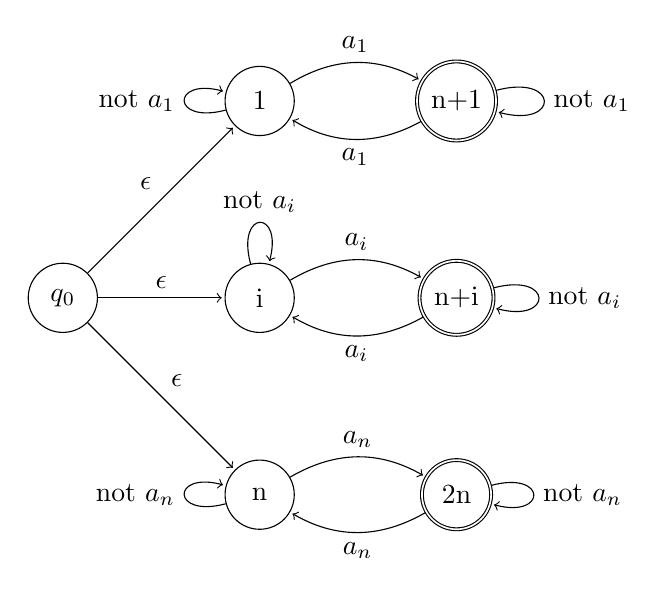
\begin{tikzpicture}[shorten >=1pt, node distance=2.5cm, on grid, auto]
  \node[state] (q0) {$q_0$};
  \node[state] (q2) [right=of q0] {i};
  \node[state] (q1) [above=of q2] {1};
  \node[state] (q3) [below=of q2] {n};
  \node[state, accepting] (q4) [right=of q1] {n+1};
  \node[state, accepting] (q5) [right=of q2] {n+i};
  \node[state, accepting] (q6) [right=of q3] {2n};
  \path[->]
  (q0) edge node {$\epsilon$} (q1)
       edge node {$\epsilon$} (q2)
       edge node {$\epsilon$} (q3)
  (q1) edge [loop left] node {not $a_1$} (q1)
  (q1) edge [bend left] node {$a_1$} (q4)
  (q4) edge [loop right] node {not $a_1$} (q4)
  (q4) edge [bend left] node {$a_1$} (q1)
  (q2) edge [loop above] node {not $a_i$} (q2)
  (q2) edge [bend left] node {$a_i$} (q5)
  (q5) edge [loop right] node {not $a_i$} (q5)
  (q5) edge [bend left] node {$a_i$} (q2)
  (q3) edge [loop left] node {not $a_n$} (q3)
  (q3) edge [bend left] node {$a_n$} (q6)
  (q6) edge [loop right] node {not $a_n$} (q6)
  (q6) edge [bend left] node {$a_n$} (q3)
  ;
\end{tikzpicture}
\end{center}
\subsection*{(b)}
  We can construct a DFA $D_i$ for each language $L^i_n$, where $L^i_n$ is the
  set of all strings over $\sum$ with an odd number of $a_i$, using two states
  as shown below. Since $L_n$ is the union of all such $L^i_n$, i.e.
  $L_n = L^1_n \cup \dots \cup L^n_n$ where $n$ is the number of symbols in the
  alphabet $\sum$, we can use the cross-product construction to combine each
  DFA $D_i$ and create a DFA $D$ that accepts the language $L_n$.
  The cross-product construction creates a DFA with $2^n$ states (since there
  are 2 states per DFA $D_i$ and thus the number of states in $D$ is doubled
  with each construction or n times). Thus there exists a DFA $D$ with $2^n$
  states that accepts the language $L_n$.
  \vspace{0.5cm}
  DFA $D_i$ that accepts the language $L^i_n$:
  \newline
  \begin{center}
  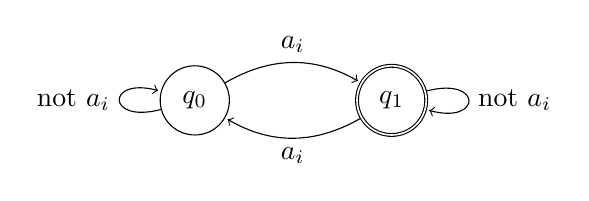
\begin{tikzpicture}[shorten >=1pt, node distance=2.5cm, on grid, auto]
    \node[state] (q0) {$q_0$};
    \node[state, accepting] (q1) [right=of q0] {$q_1$};
    \path[->]
    (q0) edge [bend left] node {$a_i$} (q1)
    (q0) edge [loop left] node {not $a_i$} (q0)
    (q1) edge [bend left] node {$a_i$} (q0)
    (q1) edge [loop right] node {not $a_i$} (q1)
    ;
  \end{tikzpicture}
  \end{center}

\subsection*{(c)}
\section*{Problem B2}
\subsection*{(a)}
\subsection*{(b)}

\section*{Problem B3}
\subsection*{(1)}
  Given that R is a regular language there DFA $D = (Q, \sum, \delta, q_0, F)$
  that accepts R i.e. $L(D) = R$. We will prove $L_1$ is regular by constructing
  an NFA $N$ using D that accepts $L_1$. Let $N = (Q \times 2^Q,
  \sum \cup \{\epsilon\}, \delta{'}, (q_0 , F), F')$ where the states in $N$
  are pairs consisting of a single state and a set of states. We define the
  transition function $\delta{'}$ as follows:
  \newline
  \indent $\forall a \in \sum$,\:$\delta{'}((p,S), a) = (\delta(p,a), S')$ where
  $S'= \{s'\,|\,\exists w \in \sum^*,\,|w| = 2,\, \delta^*(s',w) \in S\}$
  \newline
  \indent\indent i.e. the set of all states from which S is reachable via exactly
  two transitions in D.
  \newline
  We can extend $\delta{'}$ to $\delta{'}^*$ as follows:
  \newline
  \indent $\forall u \in \sum^*\: \delta{'}^* ((p,S),u) = (\delta^* (p, u),S')$
  where $S' = \{s'\:|\:\exists v \in \sum^* ,\: |v|=2|u| ,\:
  \delta^* (s', v) \in S\}$
  \newline
  \indent\indent i.e. the set of all states from which S is reachable
  via $2|u|$ transitions in D.
  \newline
  Finlly we define $F'$ as $(p, S)$ where $p \in S$ i.e. where the first element
  of the state is a member of the second element. Informally $N$ is an NFA which
  simulates traversing the DFA $D$ forwards and backwards simultaneously on any
  word $u \in \sum^*$ such that the transition function in $N$ makes one
  transition forward for each letter in $u$ starting from $q_0$ and two
  transitions backwards, starting from $F$, for every letter $a \in \sum$, thus
  accumulating a set of states that comprises the second half of a state in $N$.
  $N$ accepts a string $u$ when there exists a $v$ such that $uv \in R$ where
  $2|u| = |v|$ i.e. the state of the first element in an accepting state
  is a member of the set of states in the second element of an accepting state
  which means that $N$ ran forwards for some $u \in \sum^*$ and backwards for
  some $v \in \sum^* where 2|u| = |v|$ and ended in the same state.
  This by definition is the language $L_1$. Proof that $L(N) = L_1$:
  \newline



\subsection*{(2)}

\section*{Problem B4}
\subsection*{(a)}
  Let $D = (Q, \sum, F, q_0, \delta)$ be the DFA that accepts the regular
  language L, i.e. $L(D) = L$. We can construct a DFA for the language
  $Pre(L)$ as $D_pre = (Q, \sum, F', q_0, \delta)$ where we define $F'$
  as follows. \subsection*{(b)}
\subsection*{(c)}

\section*{Problem B5}
\subsection*{(a)} Prove that $L=L^+$ iff LL $\subseteq$ L.
\subsubsection*{Case $\implies$:}
Given $L=L^+$, prove LL $\subseteq$ L:
\newline
\begin{center}
$L = L^+ = \bigcup\limits_{n\ge1} L^n$
\newline
$LL = L^2 \subseteq \bigcup\limits_{n\ge1} L^n$
\newline
$LL = L^2 \subseteq \bigcup\limits_{n\ge1} L^n = L$
\newline
\end{center}

\subsubsection*{Case $\Longleftarrow$:}
NOTES
Given $LL \subseteq L$, prove $L^+ = L$.
\newline
Proof by induction on n where $L^+ = \bigcup\limits_{n\ge1} L^n$
Base Case: n = 1. So $L^n = L^1  = L$.
Inductive Case: Assume $L^n = L$.
Show $L^{n+1} =L$. 
\newline 
$L^{n+1} = LL^{n} = LL$. If we can show that $L \subseteq LL$, then 
$LL=L$.
STUCK. Use $(n \ge 1)$, $ \cup L^n$ to prove.
ENDNOTES

\subsection*{{b}}
($L=\emptyset$ or $L=L^*$) iff LL=L.
Recall $L^\ast = \bigcup\limits_{n \ge 0} L^n \implies L^n \subseteq L^\ast,
\forall n\ge 0$.
\newline
Case $\implies$ : Prove ($L=\emptyset$ or $L=L^*$)
$\implies LL=L$. $L = L^\ast \implies {\epsilon } \in L$
Since ${\epsilon } \in L \implies L \subseteq LL = L^2 \implies L \subseteq LL$.
From part (a) we know $L=L^+ \implies LL \subseteq L$. 
$L \subseteq LL$ and $LL \subseteq L \implies L = LL$.

Case $\Longleftarrow$ : $L=LL \implies L = L^\ast$.
(The case where $L= \emptyset$ is trivial).
Claim: $L=L^2 \implies {\epsilon } \in L$ SHOW PROOF.
By part (a), $LL=L \implies LL \subseteq L \implies
L = L^+$ and since ${\epsilon } \in L$, $L^+=L^\ast$.

\medskip
Since ${\epsilon } \in L \implies L^\ast = L^+$.
\section*{Problem B6}

\subsection*{(c)}
$ A1 = \le_1$ and $A2 = \le_2$ are wqo's.
The crossproduct ordering $(a_1,a_2) \le (b_1, b_2)
iff a_1 \le_1 b_1 and a_2 \le_2 b_2$.
Show $\le$ is also a wqo on $A_1 x A_2$.
Consider an infinite sequence $(s_i ' , s_i '') \in A_1 x A_2, i = 1,2,...$.
Have the prime sequence in A1 and have the double prime sequence in A2.
Use part (b), which says that if you have a wqo, that means the
(infinite sequence is "good") you can extend. Take first subsequence,
know it is in wqo (can extract a subsequence specified by the function f).
we knoe this subsequence is in incrasing order. use these indicies to extract
from infinite sequence.

\subsection*{(d)}
Prove the following result.
\newline
Let $n$ be any  integer such that $n>1$.
Given any infinite sequence $s_i$ with $i \ge 1$ of $n$-tuples of
natural numbers, there exist positive integers $i, j$ such that
$i<j$ and $s_{i}\preceq_{n} s_{j}$, where $\preceq_{n}$ is the
partial order on $n$-tuples of natural numbers
induced by the natural ordering $\le$ on $\mathbb{N}$
To prove: $A_i$'s are equal to $\mathbb{N}$.
So we can extend c by induction on $\preceq_{n}$ on $\mathbb{N}$.
Given that $\preceq_{n}$ is a preorder on A ($\preceq_{n} \subseteq AxA$),
then $\preceq_{n}$ is reflexive ($ x \preceq_{n} x,\forall x \in A$)
and transitive ($x \preceq_{n} y, y \preceq_{n} z \implies x \preceq_{n} z,
\forall x,y,z \in A$). NEED COMPLETE PROOF HERE.

\subsection*{(e)}
Let $\sqsubseteq$ be a preorder on a set $A$. We define the
preorder $\ll$ ({\it string embedding\/}) on $A^{*}$ as follows:
\newline
$\epsilon \ll u$ for each $u\in A^{*}$, and,
for any two strings $u=u_{1}u_{2}\ldots u_{m}$ and
$v=v_{1}u_{2}\ldots v_{n}$, $1\leq m\leq n$,
$$u_{1}u_{2}\ldots u_{m} \ll v_{1}v_{2}\ldots v_{n}$$
iff there exist  integers $j_{1},\ldots,j_{m}$ such that
$1\leq j_{1} < j_{2} < \ldots < j_{m-1} < j_{m} \leq n$ and
$$u_{1} \sqsubseteq v_{j_{1}},\ \ldots,\ u_{m} \sqsubseteq v_{j_{m}}.$$
\newline
Solution (part 1): Prove that $\ll$ is a preorder by showing (1) $u \ll u$ and
(2) $u \ll v, v \ll w \implies u \ll w$.
\newline
(1) By the definition of $\ll$, $u \ll u$ (with $u=u_{1}u_{2}\ldots u_{m}$) iff
there exist integers $j_{1},\ldots,j_{m}$ such that
$1\leq j_{1} < j_{2} < \ldots < j_{m-1} < j_{m} \leq m$ and
$u_{1} \sqsubseteq u_{j_{1}},\ \ldots,\ u_{m} \sqsubseteq u_{j_{m}}$.
This follows from definition of preorder $\sqsubseteq$ is reflexive.
\newline
(2) By the definition of $\ll$, $u \ll v$ (with $u=u_{1}u_{2}\ldots u_{m}$ and
$v=v_{1}v_{2}\ldots v_{n}$, $1\leq m\leq n$)
iff there exist integers $j_{1},\ldots,j_{m}$ such that
$1\leq j_{1} < j_{2} < \ldots < j_{m-1} < j_{m} \leq n$ and
$u_{1} \sqsubseteq v_{j_{1}},\ \ldots,\ u_{m} \sqsubseteq v_{j_{m}}.$
\newline
Additionally, by the definition of $\ll$, $v \ll w$
(with $v=v_{1}v_{2}\ldots v_{n}$ and $w=w_{1}w_{2}\ldots w_{p}$,
$1\leq n\leq p$) iff there exist integers $k_{1},\ldots,k_{n}$ such that
$1\leq k_{1} < k_{2} < \ldots < k_{n-1} < k_{n} \leq p$ and
$v_{1} \sqsubseteq w_{k_{1}},\ \ldots,\ v_{n} \sqsubseteq w_{k_{n}}$.
\newline
By the transitivity of preorder $\sqsubseteq
$, $u_{1} \sqsubseteq v_{j_{1}},\ \ldots,\ u_{m} \sqsubseteq v_{j_{m}}$
and $v_{1} \sqsubseteq w_{k_{1}},\ \ldots,\ v_{n} \sqsubseteq w_{k_{n}}
\implies u_{1} \sqsubseteq w_{k_{1}},\ \ldots,\ u_{n} \sqsubseteq w_{k_{n}}$.
And by the definition of $\ll$, $u_{1} \sqsubseteq w_{k_{1}},\ \ldots,\ u_{n}
\sqsubseteq w_{k_{n}} \implies u \ll w$.
\newline
Solution (part 2): Prove that if $\sqsubseteq $ is a partial order,
$\ll$ is a partial order, by showing that $\ll$ is anti-symmetric.
If $\sqsubseteq $ is a partial order, then it must be anti-symmetric.
Let $u=u_{1}u_{2}\ldots u_{m}$ and $v=v_{1}v_{2}\ldots v_{n}$.
Show if u $\ll$ v, and v $\ll$ u, then u = v (definition of antisymmetry).
\newline
By the definition of $\ll$, $u \ll v$ (with $u=u_{1}u_{2}\ldots u_{m}$ and
$v=v_{1}v_{2}\ldots v_{n}$, $1\leq m\leq n$) iff there exist integers $j_{1},
\ldots,j_{m}$ such that $1\leq j_{1} < j_{2} < \ldots < j_{m-1} < j_{m} \leq n$
and $u_{1} \sqsubseteq v_{j_{1}},\ \ldots,\ u_{m} \sqsubseteq v_{j_{m}}$.
By the definition of $\ll$, $v \ll u$ (with $u=u_{1}u_{2}\ldots u_{m}$ and
$v=v_{1}v_{2}\ldots v_{n}$, $1\leq n\leq m$)
iff there exist integers $j_{1},\ldots,j_{n}$ such that
$1\leq j_{1} < j_{2} < \ldots < j_{n-1} < j_{n} \leq m$ and
$v_{1} \sqsubseteq u_{j_{1}},\ \ldots,\ v_{n} \sqsubseteq u_{j_{n}}.$
\newline
Because $\sqsubseteq $ is anti-symmetric, $u_{1} \sqsubseteq v_{j_{1}},\ \ldots,
\ u_{m} \sqsubseteq v_{j_{m}}$ and $v_{1} \sqsubseteq u_{j_{1}},\ \ldots,
\ v_{n} \sqsubseteq u_{j_{n}} \implies u = v.$
\newline
Solution (part 3): Prove $\ll$ is the least preorder on $A^\ast$ satisfying:
\begin{enumerate}
\item[(1)] (deletion property)
$uv \ll uav$, for all $u, v\in A^{*}$ and $a\in A$;
\medskip
\item[(2)] (monotonicity) $uav \ll ubv$ whenever $a \sqsubseteq b$,
for all $u, v\in A^{*}$ and $a, b\in A$.
\end{enumerate}
Prove (1): Let $|uv| = m = m_1 + m_2 = |u| + |v|$, so $|uav| = m+1$.
STUCK
\newline
Prove (2): STUCK
Next, must show $u \ll v \implies u \preceq v$ for any preorder $ \preceq $ that satisfies (1) and (2).
Show that $\forall n \ge 1, \forall u_i \in \Sigma^\ast , (1 \le i \le n+1)$ and $ \forall v_i \in \Sigma^\ast (1 \le i \le n)$,
$v_1...v_n \le u_1v_1u_2...u_nv_nu_{n-1}$. Prove by induction on length of $k= |u_1|+|u_2|+ ... +|u_{n+1}|.$ 
begin office hours. Base Case: k=0 is automatic. Inductive Case: There is some $u_i$ not equal to $ \epsilon$, say $u_i = u_i ' a, a \in A$.
$u_1 ,u_2 , ... , u_i ' , ... , u_{n+1}$  so  $|u_1| + ... + |u_i '| + ... + |u_{n+1}| = k-1$. By the inductive hypothesis,
$v_1 ... v_n \le u_1 v_1 u_2 ... v_{i-1} u_i ' v_{i+1}$ by (1) end office hours.
Secondly, prove
$ \forall n \ge 1, \forall u_i \in \Sigma^\ast$ $(1 \le i \le n+1)$ and $\forall a_i,b_i \in \Sigma$ $(1 \le i \le n)$ 
if $a_i \sqsubseteq b_i, i \ge 1.$

\medskip

$u_1a_1u_2...u_na_nu_{n+1} \le u_1b_1u_2...u_nb_nu_{n+1}$ by induction on n.
Start office hours: Base Case: $n=1$. This is exactly condition two. Inductive Case: Apply the inductive hypothesis to the 
first n elements. Then set the first n elements to the value of u and apply (2) to get n + 1. end office hours
\medskip

Using these two facts for any strings u $\ll v \implies u \preceq v$ where $\preceq$ is a preorder satisfying (1) and 
(2) and $|u| \le |v|$. begin office hours: String embedding $u \ll v$ means if $u=a_1 ...a_n$, then $v=w_1 b_1 ... b_n w_{n+1}$
with $a_i \sqsubseteq b_i$ and $w_i \epsilon A^{\ast}$. So, $a_1 ... a_n  \preceq w_1 a_1 w_2 ... w_n a_n w_{n+1}$, then convert
a's to b's with proven part 2. $a_1 ... a_n  \preceq w_1 a_1 w_2 ... w_n a_n w_{n+1} \preceq w_1 b_1 w_2 ... w_n b_n w_{n+1}$
And we are done! end office hours.
\end{document}
